本附录汇集一些概率论背景知识；进一步讨论可参见教材\cite{ref38}.

先从概率测度的收敛概念开始.
\begin{definition}\label{def:B.1}\index{weak convergence@弱收敛（weak convergence）|hyperpage}
若$\mathbb R^d$上的一列概率测度$(\mu_n)_n$对所有有界连续函数$f:\mathbb R^d\to\mathbb R$都满足
$$
\int f\,d\mu_n\longrightarrow\int f\,d\mu,
$$
则称$(\mu_n)_n$（弱）收敛（weak convergence）于概率测度$\mu$.
\end{definition}

对于$\mathbb R^d$的拓扑，我们确切知道哪些子集是紧的：集合$A$紧，当且仅当它闭且有界（Heine--Borel定理）. 这给出了一个有用的判据，用来判断$A$中的序列$(x_n)_n$何时可以取子序列收敛到$A$中某一点. 下面的定义和定理刻画弱收敛拓扑下概率测度的紧集.

\begin{definition}\label{def:B.2}
若$\mathbb R^d$上的概率测度集合$\mathcal A$满足：对任意$\varepsilon>0$，都存在紧集$K$使所有$\mu\in\mathcal A$都有$\mu(K^c)\leq\varepsilon$，则称$\mathcal A$是紧的（tight）.
\end{definition}

\begin{theorem}[Prokhorov定理]\label{thm:B.3}\index{Prokhorov’s theorem@Prokhorov定理（Prokhorov’s theorem）|hyperpage}
任何弱收敛的概率测度序列都是紧的. 反之，任何紧的概率测度序列都有弱收敛子序列.

等价地，$\mathbb R^d$上的概率测度集$\mathcal A$是紧致的（compact），当且仅当它闭且紧（tight）.
\end{theorem}

我们省略证明，不过可以从一个简单例子看出其直觉：在$\mathbb R$上，令所有$n$都有$\mu_n=\delta_{x_n}$，其中$x_n\to\infty$，则$(\mu_n)_n$显然没有弱收敛子序列. 紧性（tightness）保证质量不会逃向无穷远；一旦保证这一点，就能保证存在弱收敛子序列.

下面的定理给出测度弱收敛的若干有用等价表述.

\begin{theorem}[Portmanteau定理]\label{thm:B.4}\index{portmanteau theorem@Portmanteau定理（portmanteau theorem）|hyperpage}
设$(\mu_n)_n$为$\mathcal P(\mathbb R^d)$中的序列，$\mu\in\mathcal P(\mathbb R^d)$. 下列陈述等价.
\begin{enumerate}
\item\label{item:B.4.1} $\mu_n$弱收敛于$\mu$.
\item\label{item:B.4.2} 对所有有界Lipschitz连续函数$f:\mathbb R^d\to\mathbb R$，有$\int f\,d\mu_n\to\int f\,d\mu$.
\item\label{item:B.4.3} 对所有下半连续函数$f:\mathbb R^d\to[0,\infty]$，有$\int f\,d\mu\leq\liminf_{n\to\infty}\int f\,d\mu_n$.
\item\label{item:B.4.4} 对所有上半连续函数$f:\mathbb R^d\to[-\infty,0]$，有$\int f\,d\mu\geq\limsup_{n\to\infty}\int f\,d\mu_n$.
\item\label{item:B.4.5} 对所有开集$G\subseteq\mathbb R^d$，有$\mu(G)\leq\liminf_{n\to\infty}\mu_n(G)$.
\item\label{item:B.4.6} 对所有闭集$F\subseteq\mathbb R^d$，有$\mu(F)\geq\limsup_{n\to\infty}\mu_n(F)$.
\item\label{item:B.4.7} 对所有满足$\mu(\partial A)=0$的Borel集$A\subseteq\mathbb R^d$，有$\lim_{n\to\infty}\mu_n(A)=\mu(A)$.
\end{enumerate}
\end{theorem}

\begin{proof}
\hyperref[item:B.4.1]{(1)}$\implies$\hyperref[item:B.4.2]{(2)}显然成立. 将$f$换成$-f$，容易看出\hyperref[item:B.4.3]{(3)}与\hyperref[item:B.4.4]{(4)}等价.

取补集也可知\hyperref[item:B.4.5]{(5)}与\hyperref[item:B.4.6]{(6)}等价.

\hyperref[item:B.4.2]{(2)}$\implies$\hyperref[item:B.4.3]{(3)}：已知可用一列Lipschitz连续函数$f_k:\mathbb R^d\to[0,\infty)$从下方逼近$f$. 对任意$k,n\in\mathbb N$，都有$\int f_k\,d\mu_n\leq\int f\,d\mu_n$. 令$n\to\infty$，得到$\int f_k\,d\mu\leq\liminf_{n\to\infty}\int f\,d\mu_n$. 再令$k\to\infty$，应用单调收敛定理即可.

\hyperref[item:B.4.3]{(3)}$\implies$\hyperref[item:B.4.5]{(5)}：指标函数$\mathbbm{1}_G$下半连续. 同理，由$\mathbbm{1}_F$上半连续，可得\hyperref[item:B.4.4]{(4)}$\implies$\hyperref[item:B.4.6]{(6)}.

\hyperref[item:B.4.5]{(5)}和\hyperref[item:B.4.6]{(6)}$\implies$\hyperref[item:B.4.7]{(7)}：条件$\mu(\partial A)=0$意味着$\mu(\operatorname{int}A)=\mu(A)=\mu(\overline A)$. 将\hyperref[item:B.4.5]{(5)}用于开集$\operatorname{int}A$，将\hyperref[item:B.4.6]{(6)}用于闭集$\overline A$，即证\hyperref[item:B.4.7]{(7)}.

\hyperref[item:B.4.7]{(7)}$\implies$\hyperref[item:B.4.1]{(1)}：设$f$有界且连续；不妨假设$f$非负. 注意，对$t\in\mathbb R$，有$\partial f^{-1}([t,\infty))\subseteq f^{-1}(\{t\})$，而至多只有可数个$t$能使该集合具有正的$\mu$测度. 应用\hyperref[item:B.4.7]{(7)}，得到
$$
\int f\,d\mu_n=\int_0^\infty\mu_n\{f\geq t\}\,dt
\longrightarrow\int_0^\infty\mu\{f\geq t\}\,dt=\int f\,d\mu,
$$
这里可用例如有界收敛定理来论证上述收敛，因为积分实际上可以只在有限区间上进行.
\end{proof}

下面的引理，正如其名称所示，可以把具有共同边缘的耦合“粘合”起来. 它对最优传输中的一些构造很有用，例如\autoref{prop:1.3}中Wasserstein距离三角不等式的证明.

\begin{lemma}[粘合引理]\label{lem:B.5}\index{gluing lemma@粘合引理（gluing lemma）|hyperpage}
设$\gamma,\gamma'$为$\mathbb R^d\times\mathbb R^d$上的两个测度，且对任意Borel集$A\subset\mathbb R^d$都有$\gamma(\mathbb R^d\times A)=\gamma'(A\times\mathbb R^d)$，即$\gamma$的第二边缘与$\gamma'$的第一边缘一致. 则存在三个随机变量$X,Y,Z\in\mathbb R^d$，使$(X,Z)\sim\gamma$且$(Z,Y)\sim\gamma'$.
\end{lemma}

\begin{figure}[htbp]
\centering
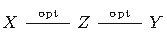
\includegraphics[width=.35\linewidth]{assets/appendixB/figB-1.pdf}
\caption{此图便于表示多个随机变量之间的耦合. 一条边表示对应耦合须最优这一约束. 一般而言，任何由无环图描述的耦合，都可以用粘合引理实现.}\label{fig:B.1}
\end{figure}

\begin{proof}
我们将明确构造这样的三元组$(X,Y,Z)$. 为此，令$Z$服从$\gamma$的第二边缘分布（根据假设，这与$\gamma'$的第一边缘相同）. 那么，$\gamma$和$\gamma'$分别确定给定$Z$时$X$和$Y$的条件分布. 例如，可以在给定$Z$时条件独立地抽取$X,Y$. 这就得到一个有效的三元组$(X,Y,Z)$，见\autoref{fig:B.1}.
\end{proof}
